% !TeX spellcheck = si_SI
% Predloga za pisanje zaključnih nalog, LADISK 2015-2018, pripravila Martin Česnik, Janko Slavič
% Zadnja verzija na: https://github.com/ladisk/latex-templates
\documentclass[12pt,a4paper,twoside,fleqn,openright]{book}

% use quite a lot of packages
\usepackage[a-3u]{pdfx}
\usepackage{amsfonts,amssymb,amsmath}
\usepackage{enumerate}
\usepackage[section]{placeins}
\usepackage{float}
\usepackage[english]{babel}
\usepackage[utf8]{inputenc}
\usepackage{graphicx}
\usepackage{ifthen}
\usepackage{fancyhdr}
\usepackage{epstopdf}
\usepackage{enumitem}
\usepackage{notoccite}
\usepackage{longtable}
\usepackage{hyperref}
\usepackage{ifoddpage}
\usepackage{tocloft}
\usepackage{titlesec}
\usepackage{pdfpages}
\usepackage{nameref}
\usepackage{multirow}
\usepackage{bm}
\usepackage{caption}
\usepackage{subcaption}
\usepackage{url}
\usepackage{icomma}
\usepackage{hyperref}
\usepackage{cite}
\usepackage[numbib]{tocbibind}
\usepackage[english]{datetime2}
\usepackage[inner=30mm,
            outer=25mm,
            top=30mm,
            bottom=25mm]{geometry}





% paragraph settings
\setlength\parindent{0pt}
\setlength{\parskip}{1.5ex plus 0.5ex minus 0.5ex}

% set equation environment indentation
\setlength{\mathindent}{0.5cm}%

% set itemize environment whitespacing and left margin
\setlist[itemize]{noitemsep,nolistsep, leftmargin=*}

% set table and figure captions
\captionsetup[table]{skip=10pt,singlelinecheck=false}
\captionsetup[figure]{justification=centering}

% set tablename to Table
%\AtBeginDocument{%
%  \renewcommand\tablename{Table}
%}

% command for multiline cell in table
\newcommand{\minitab}[2][l]{\begin{tabular}{#1}#2\end{tabular}}

% opens a new page if current page is even
\newcommand{\addifeven}{
\checkoddpage
\ifoddpage
\else
\mbox{}
\newpage
\fi}

% set section and tableofcontents depth
\setcounter{secnumdepth}{3}
\setcounter{tocdepth}{3}
\def\labelitemi{--}

%  accordingly format a chapter definition
\titleformat{\chapter}[display]
  {\bfseries}{}{0pt}{\Huge\thechapter\quad}

% set fancy_nohead fancy header
\fancypagestyle{fancy_nohead}{
\fancyhead{}
\fancyfoot[LE,RO]{\thepage}
\renewcommand{\headrulewidth}{0pt}
\chead{}
\cfoot{}
}


% assign no_header
\assignpagestyle{\chapter}{fancy_nohead}

% table, fig and eq formatting

\renewcommand{\thetable}{\arabic{chapter}.\arabic{table}}
\renewcommand{\thefigure}{\arabic{chapter}.\arabic{figure}}
\renewcommand{\theequation}{\arabic{chapter}.\arabic{equation}}

\renewcommand\cftchapdotsep{\cftdotsep}  % adds leader dots from chapter titles to page numbers

% month year date format
\DTMlangsetup{showdayofmonth=false}

\begin{document}


\pagenumbering{roman}
% !TeX spellcheck = si_SI
%Urejanje platnic, naslovnice, UDK, povzetka in kazal
%
% PLATNICA
\hypersetup{pageanchor=false} % no page anchors for the empty-pagestyle pages
% -*- TeX:SI -*-
% Platnica
\thispagestyle{empty}
\begin{center}
\large \mbox\par\par\vspace*{-0.75cm} \textbf{UNIVERSITY OF LJUBLJANA}
\\ \vspace{0.2cm} \large{Faculty of mechanical engineering}
\\ \vspace*{7cm} \LARGE{\textbf{[Design of a proposal for final assignments at the Faculty of Mechanical Engineering]}}
% without square brackets in the final version -- this applies to all fields where you enter your data (e.g. address, first and last name, date, mentor, ....)
\\ \vspace{1cm} \normalsize
% Choose the right one, delete the others
%\large{[Diploma thesis of the higher education professional study program I.~degree Mechanical Engineering]}\\
\large{[Master's thesis of the second-level master's study program Mechanical Engineering\\or\\Diploma thesis of the first-level professional study program Mechanical Engineering – Project application program]}\\
\vspace{2.5cm}
\Large{\textbf{[John Doe]}}\\
\vfill
\large{Ljubljana, [month of defense] [year of defense]}
\end{center}

\newpage

% TRI PRAZNE STRANI
\mbox{}\thispagestyle{empty}
\newpage
\mbox{}\thispagestyle{empty}
\newpage
\mbox{}\thispagestyle{empty}
\newpage

% NOTRANJA NASLOVNICA
% !TeX spellcheck = sl_SI
% Notranja naslovnica
\thispagestyle{empty}
\begin{center}
\large \mbox\par\par \vspace*{-0.75cm}\textbf{UNIVERSITY OF LJUBLJANA}
\\ \vspace{0.2cm} \large{Faculty of Mechanical Engineering}
\\ \vspace*{6.5cm} \LARGE{\textbf{[Design of a proposal for final assignments at the Faculty of Mechanical Engineering]}}
\\ \vspace{1cm} \normalsize
% Izberite pravega, ostale izbrišite
%\large{Diplomsko delo visokošolskega strokovnega študijskega programa I.~stopnje Strojništvo}\\
\large{Master's thesis of the Master's study program II.~level Mechanical Engineering}\\
\vspace{2cm}
\Large{\textbf{[John DoE]}}\\
\vspace{5cm}
\large{
Mentor: [prof. dr. Franc Horvat, univ. dipl. inž.]\\
Co-mentor: [prof. dr. Anton Kovačič, univ. dipl. inž.]
}
\vfill
\large{Ljubljana, [month of defense of thesis] [year of defense]}
\end{center}
\setcounter{page}{1} 

\newpage
\mbox{}\thispagestyle{empty}
\newpage
\hypersetup{pageanchor=true} % no page anchors for the empty-pagestyle pages

% PROSTOR ZA ODLOČBO
\thispagestyle{empty}
[Space for a signed master's thesis topic]
\newpage
\mbox{}\thispagestyle{empty}
\newpage

% PROSTOR ZA ZAHVALO
\pagestyle{fancy_nohead}
% -*- TeX:SI -*-
% Zahvala
\vspace*{0mm}
\Large\textbf{Acknowledgements}\normalsize
\vskip\medskipamount % or other desired dimension
\leaders\vrule width \textwidth\vskip0.4pt % or other desired thickness
\vskip\bigskipamount % ditto


[Writing an acknowledgment or dedication is optional.]

[In the acknowledgments, write thanks to those who helped in the creation of the work and without whom the work would not have been created in the form it is. It is usually necessary to thank first and foremost the mentor, co-mentor and the institution that may have financially or otherwise supported the completion of the final work. Then there are assistants, other colleagues and your colleagues who helped with theoretical and experimental work. Finally, we usually thank the family.]

\newpage
\mbox{}
\newpage



% IZVLEČKI IN UDK
% -*- TeX:SI -*-
% UDK in izvlečki
%
%slovenska kodna stran
\vspace*{0mm}
\Large\textbf{Izvleček}\normalsize
\vskip\medskipamount
\leaders\vrule width \textwidth \vskip0.4pt
\vspace{5mm}
\hfill UDK [123.45:678.91:234.56(789.1)]

Tek. štev.: [MAG II/99]\smallskip
\par \vspace{1cm}
\large{\textbf{[Zasnova predloge za zaključne naloge na Fakulteti za stroj\-ni\-štvo]}}\normalsize\medskip
\par \vspace{1cm}
[Janez Novak]\smallskip
\par \vspace{1cm}
Ključne besede:
\hspace{1cm}\parbox[t]{10cm}{{[}predloga{]}\\
{[}zaključna naloga{]} \\
{[}navodila{]}\\
{[}vsebina{]}\\
{[}diplomiranje{]}\\
{[}pravilnik{]}}
\par \vspace{3.5cm}


[V začetku izvlečka je jedrnat opis obravnavanega problema. Sledi opis izbrane metodologije in nato opis najpomembnejših rezultatov oz. ugotovitev brez dodatnih pojasnjevanj. Obseg izvlečka naj ne presega 200 besed oz. 600 znakov vključno s presledki.]
\newpage
\mbox{}\newpage
%
%
%angleška kodna stran
\vspace*{0mm}
\Large\textbf{Abstract}\normalsize
\vskip\medskipamount
\leaders\vrule width \textwidth\vskip0.4pt
\vspace{5mm}
\hfill UDC [123.45:678.91:234.56(789.1)]

No.: [MAG II/99]\smallskip
\par \vspace{1cm}
\large{\textbf{[Design for a template for final theses at the Faculty of Mechanical Engineering]}}\normalsize\smallskip
\par \vspace{1cm}
[Janez Novak]\bigskip
\par \vspace{1cm}
Key words:
\hspace{1cm}\parbox[t]{10cm}{{[}template{]}\\
{[}final thesis{]} \\
{[}instructions{]}\\
{[}contents{]}\\
{[}graduation{]}\\
{[}regulations{]}}
\par \vspace{3.5cm}


[Angleški prevod izvlečka\ldots]
\newpage
\mbox{}\newpage 
\newpage

% KAZALA
\vspace*{0mm}
\Large\textbf{Table of contents}\normalsize
\vskip\medskipamount
\leaders\vrule width \textwidth\vskip0.4pt
\vskip\bigskipamount

% Vsebinsko kazalo
\makeatletter
\renewcommand{\tableofcontents}{\@starttoc{toc}}
\makeatother
\tableofcontents

\newpage
\addifeven

\vspace*{0mm}
\Large\textbf{List of figures}\normalsize
\vskip\medskipamount
\leaders\vrule width \textwidth\vskip0.4pt
\vskip\bigskipamount
\addcontentsline{toc}{section}{List of figures}

% Seznam slik
\makeatletter
\renewcommand{\listoffigures}{\@starttoc{lof}}
\makeatother
\renewcommand\cftfigpresnum{Figure~}
\renewcommand\cftfigaftersnum{:}

\newlength{\mylen} % a "scratch" length
\settowidth{\mylen}{\bfseries\cftfigpresnum\cftfigaftersnum} % extra space
\addtolength{\cftfignumwidth}{\mylen} % add the extra space
\setlength{\cftfigindent}{0pt}

\listoffigures



\newpage
\addifeven

\vspace*{0mm}
\Large\textbf{List of tables}\normalsize
\vskip\medskipamount
\leaders\vrule width \textwidth\vskip0.4pt
\vskip\bigskipamount
\addcontentsline{toc}{section}{List of tables}
% Seznam tabel
\makeatletter
\renewcommand{\listoftables}{\@starttoc{lot}}
\makeatother

\renewcommand\cfttabpresnum{Table }
\renewcommand\cfttabaftersnum{:}
\settowidth{\mylen}{\bfseries\cfttabpresnum\cfttabaftersnum} % extra space
\addtolength{\cfttabnumwidth}{\mylen} % add the extra space
\setlength{\cfttabindent}{0pt}

\listoftables

\newpage 


\newpage
% !TeX spellcheck = si_SI
\addifeven

\vspace*{0mm}
\Large\textbf{List of used symbols}\normalsize
\vskip\medskipamount
\leaders\vrule width \textwidth\vskip0.4pt
\vskip\bigskipamount

\addcontentsline{toc}{section}{List of used symbols}
\begin{longtable}[l]{@{}p{.15\textwidth}@{}p{.15\textwidth}@{}p{.7\textwidth}@{}}
\hline
Symbol & Unit & Meaning\\
\hline
\endfirsthead
\hline
\endhead
&&\\
$A$ & m$^2$ & area\\
$C$ & / & concentration \\
$D$ & m$^2$s$^{-1}$ & diffusion coefficitent\\
$d$ & mm & premer \\
$P$ & Pa, bar & tlak \\
$V$ & m$^3$ & volumen\\
&&\\
$\nu$ & m\,s$^{-1}$ & hitrost\\
$\gamma$ & m$^2\,$l$^{-1}$ & stopnja povečevanja mašenja\\
$\varepsilon$ & / & učinkovitost\\
$\eta$ & Pa\,s & dinamična viskoznost\\

\end{longtable}


\begin{longtable}[l]{@{}p{.15\textwidth}@{}p{.85\textwidth}@{}}
\hline
Indices & \\
\hline
\endfirsthead
\hline
\endhead
&\\
ent & entire\\
f & filtration\\
k & koncentrat\\
p & permeat\\
z & začetni\\
\end{longtable}

\newpage

\addifeven

\vspace*{0mm}
\Large\textbf{List of used acronyms}\normalsize
\vskip\medskipamount
\leaders\vrule width \textwidth\vskip0.4pt
\vskip\bigskipamount

\addcontentsline{toc}{section}{List of used acronyms}

\begin{longtable}[l]{@{}p{.2\textwidth}@{}p{.8\textwidth}@{}}
\hline
Acronym & Meaning\\
\hline
\endfirsthead
\hline
\endhead
&\\
ACH & aluminijev clorohydrate, type of coagulant\\
COD$_{\text{Mn}}$ & ekvivalent kisika, potrebnega za oksidacijo organske vsebine vzorca z uporabo trivalentnega mangana (ang. \emph{Chemical Oxygen Demand})\\
GAC & aktivno oglje v granulah (ang. \emph{Granular Activated Carbon})\\
MF & mikrofiltracija\\
NF & nanofiltracija\\
PAC & aktivno oglje v prahu (ang. \emph{Powder Activated Carbon})\\
RO & reverzna osmoza\\
SCADA & sistem za nadzor in zajemanje podatkov (ang. \emph{Supervisory Control And Data Acquisition})\\
TOC & skupna količina vseh organskih spojin v vzorcu (ang. \emph{Total Organic Carbon})\\
TSS & količina vseh suspendiranih trdnih delcev v vzorcu (ang. \emph{Total Suspended Solids})\\
UF & ultrafiltracija\\
\end{longtable}

\newpage

\newpage \mbox{}
\addifeven
\newpage

%change header and foot for non-chapter pages

\renewcommand{\chaptermark}[1]{\markboth{#1}{}}

\fancyhf{}
\fancyhead[RO]{\nouppercase{\leftmark}}
\fancyhead[LE]{\nouppercase{\leftmark}}
\fancyfoot[LE,RO]{\thepage}
\renewcommand{\headrulewidth}{0.1mm}
\renewcommand{\footrulewidth}{0mm}
\cfoot{}
\setlength{\headheight}{15pt}

\pagestyle{fancy}

\pagenumbering{arabic}

% !TeX spellcheck = si_SI
\chapter{Introduction}\label{cha:introduction}

\section{Problem background}\label{sec:problem_background}
The introductory chapter should contain two subsections: \ref{sec:background_of_the_problem} \nameref{sec:background_of_the_problem} and \ref{sec:goals_of_tasks} \nameref{sec:goals_of_tasks}. The chapter \ref{sec:background_of_the_problem} \nameref{sec:background_of_the_problem} should contain at least one introductory paragraph, where there should be a general description or explanation of the discussed topic. Present the starting points of the final work and its importance.


\section{Task Objectives}\label{sec:Task_Objectives}
Present the problems, goals and structure (description of content, division by chapters) of the final work in a special sub-chapter.

Do not present results and conclusions in the introduction. In this section, focus on what will be presented in the work and how the work is structured. Write what you will do, what you expect from theoretical and what from practical research, and what are the risks and dangers of not achieving these goals. Write about hypotheses, not results.

\section{Instructions for using the template for final assignments}\label{sec:using_the_template}
In this proposal, in the non-content part of the final assignment (up to page xxii), the part of the text that the student or student to change it to suit his or her data and data about his or her final assignments. Since you are using \LaTeX~, the Table of Contents, Table of Figures and Table of Contents are updated every time you compile.

In this proposal, in the substantive part of the final thesis, there are instructions and examples for creating the final thesis. The entire text (the main titles remain: \nameref{cha:introduction}, \nameref{cha:teoreticne_osnove}, etc.) must be read by the student or replace the student with a text that corresponds in content to his or her final assignments.

\subsection{Using preset styles in a template}\label{sec:presets}
To write the final paper, use this template, which already contains \textbf{preset styles} to unify the final form of final papers on FS.

As you can see from the template, you use the following commands for addresses:
\begin{itemize}
\item \verb|\chapter| for main titles,
\item \verb|\section| for a Level 2 title,
\item \verb|\subsection| for a level 3 title,
\item \verb|\subsubsection| for a level 4 title,
\item \verb|\begin{itemize}\item\end{itemize}| to indent.
\end{itemize}

For \textbf{titles of figures and tables} (and also the numbering of equations) use the automatic numbering option, either below the figure or above the table. You define the title of the figure or table with the command \verb|\caption{<>}|, the label of the figure, equations and tables is defined with \verb|\label{<>}|, and you refer to them with \verb|\ref{< >}| or to equations with \verb|\eqref{<>}|. This method enables easy automatic numbering of images and tables (e.g. no need to manually correct the numbering if you insert a new image or table in the text) and also easy creation of a list of images or list of spreadsheets. \LaTeX these macros ensure that all numbered fields are automatically updated during compilation, including lists in the non-content section.

To insert an equation such as equation \eqref{eqn:e} in chapter \ref{sec:enacbe} \nameref{sec:enacbe}, use environment \verb|\begin{equation}<>\end{equation}|.

\subsection{References to parts of the text}\label{sec:references}

Referring to a figure, table, equation or piece of text is quite easy and unambiguous in \LaTeX. Please note that when referring to the image or spreadsheet, use a lowercase initial, e.g. \verb|image \ref{<>}|. When referring to an equation, also use a lowercase letter and place the equation number in brackets, e.g. \verb|equation \eqref{<>}|.




\newpage


% !TeX spellcheck = sl_SI
\chapter{Theoretical foundations and literature review}\label{cha:theoretic_foundations}

\section{Content}\label{sec:content}
Regardless of whether the task is theoretically or experimentally oriented, it is
it is necessary to first process the theoretical foundations of the discussed topic.

\subsection{Source of information}\label{sec:source_of_information}
When reviewing the literature, the books should be primarily professional and scientific
articles the main source of information. When searching for articles and other literature online
we recommend using the following search engines: Dikul, Web of Science, ScienceDirect
and Google Scholar.

Read more about citing sources later in this template.

\section{Subsections and styles}\label{sec:subsections}
Divide the individual parts sensibly into sub-chapters, which should be consecutive
numbered. The format and style of headings should correspond to those shown in this
suggestions. The numbering should be automatic as shown in this template.
Use this template directly to write your final paper, as all styles are
already preset (regular style, style for chapters and sub-chapters, style for
titles of tables and pictures, etc.).

\subsection{Level 2 Subchapter}\label{sec:chapter_2}
\subsubsection{Level 3 Subchapter}\label{sec:chapter_3}

The first lines of paragraphs should not be indented, but should be indented
paragraphs with one blank line each. Between the title of the subsection and the end of the previous one
the text should be 2 blank lines apart. If the subsection title begins
immediately after the heading of the higher-level subchapter, there should be no blanks between the headings
lines. You can use a maximum of 4 levels of addresses, i.e. the main address and the 3rd
subtitle level.

\textbf{Additional text delimitation}\\
If you want to further separate individual parts in the last, 4th level of the subsection
text, you can use one line of bold \verb|\textbf{<>}|.

\subsubsection{Using bold, italic and underline
print}\label{sec:emphasis_types}

In addition to the previous example, the use of \textbf{bold} makes sense:
\begin{itemize}
\item when we first mention and define the very important term for in the text
understanding the task,
\item when we want to emphasize a particular part or thought,
\item when we want e.g. clearly separate individual parts of the text when enumerating.
\end{itemize}

When words from foreign languages are used in the text, we use italics or
cursive print (eng. \emph{italics}). \underline{Underlined print} generally not
we use


\subsubsection{Enumeration Levels}\label{sec:itemizing}

No matter how many hierarchical levels of indentation are used in the text for
enumeration (usually no more than 2), we always use the same throughout the text
the combination and the way of marking individual levels of indents. With this we achieve
uniform appearance of the text.

To indicate all levels of indents, we use the sign "--". Editing margins
we leave the pages for each level to \LaTeX u. An example is shown below:
\begin{itemize}
\item level 1 example:
\begin{itemize}
\item level 2 example,
\item level 2 example,
\end{itemize}
\item level 1 example:
\begin{itemize}
\item level 2 example,
\item level 2 example.
\end{itemize}
\end{itemize}

Before a new paragraph of text, there should be 1 blank line after the last indent
space, or 2 blank lines of space if the last indent is followed by a title
of a new chapter.

\section{Spreadsheets}\label{sec:spreadsheets}

Tables should be numbered consecutively, which is automatically taken care of by \LaTeX.
The spreadsheet should be centered. An example is shown in the table
\ref{tab:efficiency_of_processes}.

The title of the spreadsheet with the serial number of the spreadsheet and a short description should be
above the spreadsheet. The short description of the spreadsheet should start with a capital letter and
end with a final punctuation mark. There should be a 1 between the text and the spreadsheet title
(blank) line space, as in a spreadsheet
\ref{tab:ucinkovitost_procesov}, unless the title of the spreadsheet is at the very top
pages. There should be 2 empty lines between the table and the continuation of the text.

\begin{table}[ht!]
\caption{Efficiency of different removal processes
o\-nes\-na\-al\-val\-pipe of water \cite{bazant_1991}.}
\label{tab:efficiency_of_processes}
\centering
\begin{tabular}{|l|@{}c|@{}c|@{}c|@{}c@{}|}
\hline
\multirow{4}*{\minitab[c]{Process}} &
\multirow{4}*{\minitab[c]{Removal\\micro-\\organisms}} &
\multirow{4}*{\minitab[c]{Removal\\suspended\\substances}}&
\multirow{4}*{\minitab[c]{Removal\\dissolved\\inorganic\\substances}}&
\multirow{4}*{\minitab[c]{Removal\\dissolved\\organic\\substances}}\\
&&&&\\
&&&&\\
&&&&\\
\hline
\textbf{Biological}&&&&\\
\hline
\quad Active &
\multirow{2}*{\minitab[c]{+}} &
\multirow{2}*{\minitab[c]{+}} &
\multirow{2}*{\minitab[c]{-}} &
\multirow{2}*{\minitab[c]{+}}\\
\quad mud & & & &\\
\hline
\quad Anaerobic &
\multirow{2}*{\minitab[c]{-}} &
\multirow{2}*{\minitab[c]{+}} &
\multirow{2}*{\minitab[c]{-}} &
\multirow{2}*{\minitab[c]{+}}\\
\quad processing & & & &\\
\hline

\quad Biofilters & - & - & - & +\\
\hline
\textbf{Chemical}&&&&\\
\hline
\quad Chlorination & + & + & - & +\\
\hline
\quad Ozonation & + & + & - & $\circ$\\
\hline
\quad Coagulation & + & + & - & +\\
\hline
\textbf{Physical}&&&&\\
\hline
\quad Adsorption &
\multirow{2}*{\minitab[c]{}} &
\multirow{2}*{\minitab[c]{}} &
\multirow{2}*{\minitab[c]{}} &
\multirow{2}*{\minitab[c]{}}\\
\quad per active. charcoal:& & & &\\
\hline
\quad \quad in granules & - & + & - & +\\
\hline
\quad \quad in powder & + & + & - & +\\
\hline
\quad Conventional &
\multirow{2}*{\minitab[c]{-}} &
\multirow{2}*{\minitab[c]{+}} &
\multirow{2}*{\minitab[c]{-}} &
\multirow{2}*{\minitab[c]{-}}\\
\quad filtration& & & &\\
\hline
\quad Flocculation&
\multirow{2}*{\minitab[c]{+}} &
\multirow{2}*{\minitab[c]{+}} &
\multirow{2}*{\minitab[c]{-}} &
\multirow{2}*{\minitab[c]{-}}\\
\quad + sediment. &&&&\\
\hline
\quad Membrane&
\multirow{2}*{\minitab[c]{}} &
\multirow{2}*{\minitab[c]{}} &
\multirow{2}*{\minitab[c]{}} &
\multirow{2}*{\minitab[c]{}}\\
\quad processes&&&&\\
\hline
\quad \quad MF & + & + & - & -\\
\hline
\multicolumn{5}{l}{\scriptsize{Legend: + removal in progress
efficient, $\circ$ removal partially takes place, - removal does not
in progress}} \\
\end{tabular}
\end{table}

If a table or part of a table is taken from another source, it is required
to quote. If the entire table is summarized, the reference number is written k
description of the spreadsheet. If only certain values or text within are summarized
cells, this can be quoted in individual cells or at the end of an individual line.

Tables must be legible, clear and transparent. Under a spreadsheet or image
can be done with a smaller font size \verb|\footnotesize| or \verb|\scriptsize|
write down any notes or e.g. legend as shown in the table
\ref{tab:efficiency_of_processes}. All tables and figures must be
(previously) mentioned in the text and also explained in more detail.

The table should be sensibly placed in the text. We usually place the spreadsheet
under the paragraph in which the spreadsheet is mentioned for the first time. If the spreadsheet because of more
of the fluid formatting of the text is placed differently, it should definitely be placed in
near the first mention in the text.

If possible, we display each spreadsheet (or image) on one page. If
due to the size of the spreadsheet, it is not possible to avoid dividing it into several pages,
at the end of each page (if the table continues on the next page) to the right
write "to be continued" below, to the next page (where the spreadsheet
continues) and "continuation" in the top left. Be sure to repeat on each page
print the entire header of the spreadsheet, and number the columns if necessary. For such
cases it makes sense to use the \verb|longtable| package as already used in v
List of used symbols.

\section{Images}\label{sec:images}

Images should be numbered consecutively, which is automatically taken care of by \LaTeX. A picture
should be centered. An example is shown in the figure
\ref{fig:image_microscope}.

\begin{figure}[ht!]
\begin{centering}
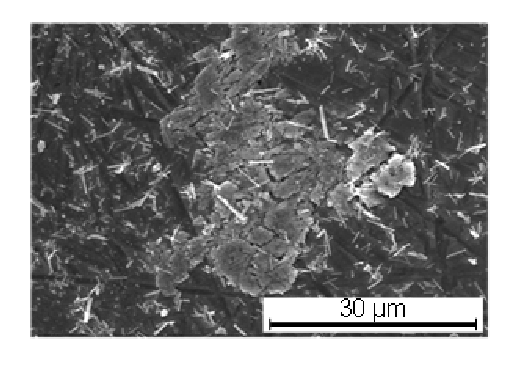
\includegraphics[scale=1.0]{figures/slika_mikroskop}
\caption{Image taken with an electron microscope
\cite{stropnik_1997}.}
\label{fig:picture_microscope}
\end{centering}
\end{figure}

\begin{figure}[ht!]
\begin{centering}
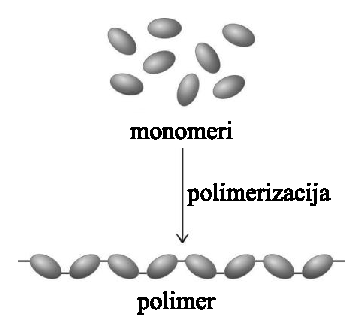
\includegraphics[scale=1.0]{figures/neke_molekule}
\caption{Schematic representation of the polymerization process
\cite{stropnik_1997,Doe_1991}.} \label{fig:some_molecules}
\end{centering}
\end{figure}

The title of the image with the serial number of the image and a short description should be below the image,
centered with respect to the image and text. The image description should start with a capital
initial and ends with a final punctuation mark. It is recommended that the names or
the descriptions of the pictures (as well as the tables) are short, as it is from the point of view of later production
index of images (or spreadsheets) is more appropriate.

Images must be legible, clear and transparent. The pictures must be good
quality and in the Slovenian language. If there is a diagram in the picture, there must be magnitudes
and units of all axes clearly and consistently marked. In microscopic images, it must
be a properly marked length scale. Images that are mapped with optical
readers should be in the best possible resolution. Pictures that you create yourself with
programs such as CorelDraw, Photoshop, PowerPoint, etc. should be saved in
*.emf (Enhanced Metafile) or *.eps (Encapsulated
PostScript). In this way, they will be when converting the document to *.pdf format
preserved all the details in the image and will also be guaranteed when printing
the highest possible quality.

Each image (e.g. also the images \ref{fig:neke_molekule} and \ref{fig:2_graph}) should
will be meaningfully placed in the text. We usually place the image below the paragraph, v
which we mention her for the first time. If the image due to more fluid formatting of the text
placed differently, it should definitely be placed near the first mention in the text. If
the pictures are placed one below the other, they should be between the title of the first picture and drugo
picture 2 empty lines.

\begin{figure}
\begin{subfigure}[b]{.45\linewidth}
\centering 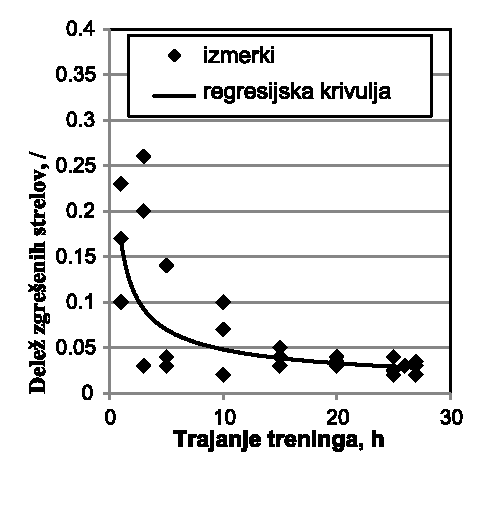
\includegraphics[scale=0.7]{figures/graf_1}
\caption{}\label{subfig:graph1}
\end{subfigure}%
\quad
\begin{subfigure}[b]{.45\linewidth}
\centering 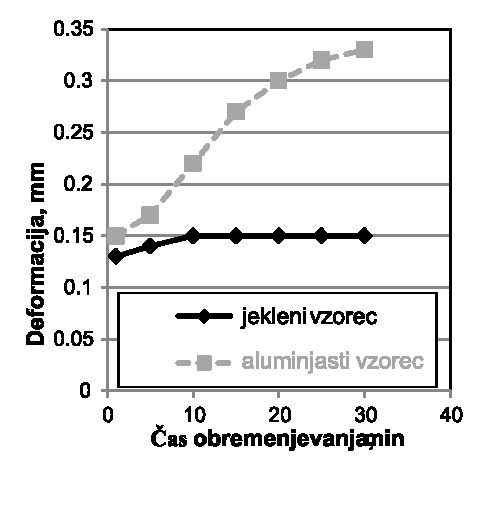
\includegraphics[scale=0.7]{figures/graf_2}
\caption{}\label{subfig:graph2}
\end{subfigure}

\caption{(a) Dependence of the proportion of missed shots in the addiction competition
from the training time preceding it and (b) deformation as a function of time
loads for two different samples.}\label{fig:2_graph}
\end{figure}

\begin{figure}[ht!]
\begin{centering}
\includegraphics[scale=1.0]{figures/voda_in_nekej}
\caption{Time sequence of a projectile falling into water from a height of (a) 2.1 m;
and (b)
4.1 m \cite{Loukides_2020}.} \label{fig:voda_in_nekej}
\end{centering}
\end{figure}

As shown in the pictures \ref{fig:2_graph} and \ref{fig:voda_in_nekej}, you can
combine several related diagrams into one image, clearly separating them on
subassemblies, i.e. (a) and (b), while paying attention to transparency.

If the image is taken from a specific source, it must be cited as such
shown in the picture \ref{fig:picture_microscope}. Also all pictures by other authors
must be cited.

\section{Equations}\label{sec:equations}

Formulation of the equation is automatic in \LaTeX. The explanation of the equation must be in
to the text.
\begin{equation}\label{eqn:e}
e = m\,c^2
\end{equation}
\begin{equation}\label{eqn:e_cel}
e_{\text{cel}}=\sum_{i=1}^{n}\,m_{i}c^2
\end{equation}
\begin{equation}\label{eqn:2NZ}
	\sum_{i=1}^{N}\bm{F}_i(t)=m\,\ddot{\bm{r}}(t)
\end{equation}

In the rest of the text, if necessary, reference is made to the corresponding number
equations, e.g. to the equation \eqref{eqn:e}.

We usually use Latin and Greek letters for size labels and other symbols
alphabet, sometimes with the addition of indices and other characters. As shown in Eqs
\eqref{eqn:e_cel} and \eqref{eqn:2NZ}, must be symbols, i.e. labels of quantities,
e.g. $e$ or $m$, written in italics. Furthermore, symbols for vector quantities should be written in italic bold. Not behind the symbol
we place dots, unless the sentence ends with a symbol.

Indices are usually used when two quantities have the same symbol, or if
we want to define the quantity additionally (e.g. $_{\text{max}}$ as the largest,
$_{\text{cel}}$ as whole, $_{\text{z}}$ as initial, etc.). Indexes that
denote physical quantities, written in italics, descriptive
indexes that serve for additional definition of quantities, e.g. "whole" v
$e_{\text{cel}}$ or "L" in $Pr_{\text{L},i}$ must be written in normal
(vertical) press. We also write indices that consist of numbers in
to normal (upright) print (e.g. $A_1$), subscripts from letters denoting counts
or numbers (e.g. "i" in $m_i$ or in $Pr_{\text{L},i}$) are written in italics
(italic) print.

For correct specification of physical quantities, constants, indices and others
elements in the equations, please note the "Recommendations to the authors of academic and professional
of publications at the Faculty of Mechanical Engineering in Ljubljana" by the author
senior lecturer~dr.~Stropnik \cite{stropnik_1997}.

\section{Citing and citing sources}\label{sec:citing}

When citing sources, use the Slovenian version of the IEEE standard. Citation
or citation of sources does not only apply to final works, but also in general to
any representation in which intellectual or material are used
property of other authors. Use as many resources as possible
\textbf{newer relevant international professional} literature. Online resources
pages/internet can represent \textbf{maximum 25\%} of all resources,
used in the final part (not articles).

The IEEE standard is mainly used in computer, electrical,
telecommunications and engineering fields. Each contains three basic data
source:
\begin{itemize}
\item The author, who is written as the first letter of the name and the full last name, (J.
Novak).
\item Title of article, patent, conference paper,... in duplicate
they dictate ("Modal analysis").
\item Journal or book title in italics (\emph{Stability of
Structures: Elastic, Inelastic, Fracture, and Damage Theories})
\end{itemize}
Thus, the reader quickly finds the source of the information. All data, pages, collections,
editions... differ from each other depending on the type of resource and are required
several times to find out additionally.

All used literature is listed in the text of the assignment in order
numbers in \textbf{square brackets}, so there should also be a list of the bibliography
numbered according to the order in which the citations appear in the document. There are examples
shown in the following sentences:
\begin{itemize}
\item An overview is given in the work of Bažant and colleagues \cite{bazant_1991}
influences on the stability of structures. \emph{You can also:}
\item In the work of Bažant et al. \cite{bazant_1991} an overview of the influences on
stability of structures.
\item In 2008, Bažant and Cedolin \cite{Bazant_2008} presented
the use of modal analysis in analyzing the stability of structures.
\item The model is listed in \cite{Doe_1991}. (\emph{it is not necessary to write: "vliterature \cite{Doe_1991}«}.)
\item When citing several works, it is recommended that they be separated by square brackets
brackets e.g.: ...recalculation of the model was used by \cite{bazant_1991},
\cite{Doe_1991}, \cite{Bazant_2008}; (also acceptable
\cite{bazant_1991,Doe_1991,Bazant_2008})
\item When you quote several works and they follow one another, e.g. ...economical
the impact on performance is pursued by \cite{bazant_1991}-\cite{Bazant_2008};
(also acceptable \cite{bazant_1991, stropnik_1997,
Doe_1991,Loukides_2020, Bazant_2008})
\end{itemize}

The serial number of the source cited in square brackets is
repeated in the list of literature (see \ref{sec:zzorci_lit}
\nameref{sec:zzorci_lit}), when referring to the same reference again later
but we use the same number as for the first reference. All this is in \LaTeX u
performed automatically, but the final control is definitely not superfluous.

The list of used literature should be left aligned (eng. align left) and
designed according to the examples in this template (see chapters \ref{sec:examples_lit}
\nameref{sec:zzorci_lit} and 7 Literature).

When referring to a source, we can use "et
al.", for example: In the work of Bažant et al. \cite{bazant_1991} an overview is given
of influences\ldots

Samples of the bibliography are given below. By specifying the listed and (or)
other relevant data from sources, such as: conference papers,
patents, standards, regulations, prospectuses, studies, other diplomas, or at
When citing literature, please also consider:
\begin{itemize}
\item SIST ISO 690: 1987(E) Documentation – Bibliographic references:
Content, form and structure; and
\item SIST ISO 690 – 2 : 1997(E) : Electronic documents or parts thereof.
\end{itemize}


\subsection{Samples of literature list}\label{sec:zzorci_lit}

\textbf{For books:}
\begin{itemize}
\item[{[1]}] Z.~P. Ba\v{z}ant and L.~Cedolin, \emph{Stability of Structures:
Elastic, Inelastic, Fracture, and Damage Theories}.\hskip 1em plus
0.5em minus
0.4em\relax New York: Oxford University Press, 1991.\\

\item[{[2]}]J.~Stropnik, \emph{Recommendations to authors of study and
professional
publications at the Faculty of Mechanical Engineering in Ljubljana}.\hskip 1em plus
0.5em minus
0.4em\relax Ljubljana: Faculty of Mechanical Engineering, 1997.
\end{itemize}

\textbf{For book chapters:}
\begin{itemize}
\item[{[3]}] J.~Doe, ``Earthquake stability,'' in \emph{Stability of
Structures:
Elastic, Inelastic, Fracture, and Damage Theories}, Z.~P. Pheasant and
L.~Cedolin,
ed.\hskip 1em plus 0.5em minus 0.4em\relax New York: Oxford University
Press,
1991, p. 124--157.
\end{itemize}

\textbf{For e-books:}
\begin{itemize}
\item[{[4]}] M.~Loukides and J.~Bruner, \emph{Building a Solid World},
1st edition,
Beijing, O'Reilly, [e-book], 2014. Available at:
\url{https://doi.org/10.1093/acprof:oso/9780199343638.003.0004} [view 10
June 2020].
\end{itemize}

\textbf{For magazines:}
\begin{itemize}
\item[{[5]}] Z.~P. Ba\v{z}ant and L.~Cedolin, ``Noise control,'' \emph{J.
Sound
Vib.}, No. 111, p. 42--50, 2008.\\
\item[{[6]}] J.~Gonzalez-Gutierrez, J.~L. Carillo-Estrada and J.~C.
Ruiz-Suarez,
``Penetration of granular projectiles into a water target,''
\emph{Scientific
reports}, vol.~4, no. 6762, p. 1--5, 2014.
\end{itemize}

\textbf{For conference papers:}
\begin{itemize}
\item[{[7]}] Z.~P. Ba\v{z}ant and L.~Cedolin, ``Modal analysis,'' in
\emph{Kuhljevi dnevi: Zbornik referatov}, B.~Podskrajnik (ed.), Ljubljana,
2005, p. 2--5.\\

\item[{[8]}] Z.~P. Ba\v{z}ant and L.~Cedolin, ``Modal analysis,'' v
\emph{Proceedings of the 22nd Congress of Polymers}, S.~Smith (ed.), London,
2007, p. 3--8.\\
\end{itemize}

\textbf{For online resources with a known author:}
\begin{itemize}
\item[{[9]}]C.~Kogoj, \emph{Modal analysis: selected chapters from {DTD}}.
accessible at:
\url{http://lab.fs.uni-lj.si/ldtd/Gradivo_za_studente/DTD/Pregled\%20teorije.pdf}
[view: 11/01/2012].
\end{itemize}

\textbf{For publications of organizations (printed or published on the web
pages):}
\begin{itemize}
\item[{[10]}] \emph{Annual report of the company {M}erkur d.d. {K}ranj}, {Mercury
d.d., Kranj}, 2005.\\

\item[{[11]}] \emph{{Statistical yearbook of the Republic of Slovenia 2009}},
Statistical Office of the Republic of Slovenia, Ljubljana, 2009.\\

\item[{[12]}]\emph{Standard Classification of Activities 2005}, {Statistical
office
Republic of Slovenia}. accessible at:
\url{http://www.stat.si/klas/tabela.aspx?cvn=1895}
[view: 10/01/2012].
\end{itemize}

\textbf{For websites of organizations, societies, individuals:}
\begin{itemize}
\item[{[13]}] \emph{M Kariera - Employment portal}. accessible at:
\url{http://www.mercator.si/kariera} [view: 10/01/2012].
\end{itemize}

\textbf{For online databases, encyclopedias, dictionaries, etc.:}
\begin{itemize}
\item[{[14]}] ``Engineering,'' in \emph{Encyclopedia Britannica online}.
accessible at:
\url{http://student.britannica.com/comptons/article-9274119/engineering}
[view: 8/1/2012].\\

\item[{[15]}] ``Business Application,'' in \emph{eSlovar}. accessible at:
\url{http://www.eslovar.com/besedilo.asp?id=1563} [viewed: 8 January 2012].
\end{itemize}

\textbf{For legislation (official documents, regulations, standards):}
\begin{itemize}
\item[{[16]}] \emph{Act on Commercial Companies}, Official Gazette of the RS no.
42/2006, 60/2006 app., 26/2007-ZSDU-B, 33/2007-ZSReg-B, 67/2007-ZTFI
(100/2007
app.), 10/2008, 68/2008, 23/2009; Sec. US: U-I-268/06-35.\\

\item[{[17]}] \emph{Act on Environmental Regulations}, Official Gazette of the RS no.
72/2009-UPB2, 65/2010.\\

\item[{[18]}] {ISO 2573:1977}: \emph{Tensile testing systems –
Determination of
K-value}, {ISO 2573:1977}.\\

\item[{[19]}] \emph{Determination of surface roughness values R$_a$, R$_z$,
R$_{max}$}, {DIN 4768:1990}.\\

\item[{[20]}] \emph{Geometrical product specifications (GPS) profile method
–
Terms, definitions and surface texture parameters}, {JIS B 0601:2001}.
\end{itemize}

\textbf{For doctoral theses and other final works:}
\begin{itemize}
\item[{[21]}] A.~Novak, \emph{Manufacturing an automated peeling machine
krompirja}, doctoral dissertation, Ljubljana, 2015.
\end{itemize}

The bibliography is performed automatically in \LaTeX, based on your database
bibliography (which, in the case of a proposal, is located at References.bib) and selected
macros that generate the \TeX~bibliography syntax accordingly. For finishing works on
For the Faculty of Mechanical Engineering, a corresponding macro has been prepared, which is located in
fs\_final\_tasks.bst. You define its use with a command
\verb|\bibliographystyle{IEEEtran_slo}| in the main file.

References to the literature inventory are automatically generated, e.g.: \cite{bazant_1991},
\cite{Doe_1991}, \cite{Bazant_2008}, \cite{Gonzalez_2014, Bazant_2005}
\cite{Bazant_2007, Kogoj_DTD, Merkur_2005, SURS_2009, SURS_2005, MKariera,
Encyclopedia, Posl_app, ZGD, ZOP}, \cite{ISO_2573}, \cite{DIN_4768} and
\cite{JISB0601, Novak_2015}.

\newpage


% !TeX spellcheck = si_SI
\chapter{Research methodology}\label{cha:methodology}

In this chapter, depending on the type of task (research or development), present, explain and justify the used \textbf{methods or procedures} measurements, calculations, modeling procedures, etc. and present and justify the selection of \textbf{materials and samples} used. In this chapter, also elaborate on measurement uncertainty.

\section{Calculations}\label{sec:calculations}

Based on the assumptions about \ldots, we used the derivation \ldots Lorem ipsum dolor sit amet, consectetur adipiscing elit, sed do eiusmod tempor incididunt ut labore et dolore magna aliqua to calculate \ldots. Ut enim ad minim veniam, quis nostrud exercise ullamco laboris nisi ut aliquip ex ea commodo consequat. Duis aute irure dolor in reprehenderit in voluptate velit esse cillum dolore eu fugiat nulla pariatur. Excepteur sint occaecat cupidatat non proident, sunt in culpa qui officia deserunt mollit anim id est laborum.

\section{Experimental part}\label{sec:experiment}
\subsection{Samples and Materials}\label{sec:samples}
\subsubsection{Gear pair}\label{sec:gear_pair}
For the gear pair we chose \ldots Lorem ipsum dolor sit amet, consectetur adipiscing elit, sed do eiusmod tempor incididunt ut labore et dolore magna aliqua. Ut enim ad minim veniam, quis nostrud exercise ullamco laboris nisi ut aliquip ex ea commodo consequat. Duis aute irure dolor in reprehenderit in voluptate velit esse cillum dolore eu fugiat nulla pariatur. Excepteur sint occaecat cupidatat non proident, sunt in culpa qui officia deserunt mollit anim id est laborum.

\subsubsection{Gred}\label{sec:gred}
The shaft was made of \ldots Lorem ipsum dolor sit amet, consectetur adipiscing elit, sed do eiusmod tempor incididunt ut labore et dolore magna aliqua. Ut enim ad minim veniam, quis nostrud exercise ullamco laboris nisi ut aliquip ex ea commodo consequat.


\subsection{Test methodology}\label{sec:methodology}
\subsubsection{Zobn experiment}\label{sec:zobn_experiment}
We designed \ldots Lorem ipsum dolor sit amet, consectetur adipiscing elit, sed do eiusmod tempor incididunt ut labore et dolore magna aliqua. Ut enim ad minim veniam, quis nostrud exercise ullamco laboris nisi ut aliquip ex ea commodo consequat. Duis aute irure dolor in reprehenderit in voluptate velit esse cillum dolore eu fugiat nulla pariatur. Excepteur sint occaecat cupidatat non proident, sunt in culpa qui officia deserunt mollit anim id est laborum.

Lorem ipsum dolor sit amet, consectetur adipiscing elit, sed do eiusmod tempor incididunt ut labore et dolore magna aliqua. Ut enim ad minim veniam, quis nostrud exercise ullamco laboris nisi ut aliquip ex ea commodo consequat. Duis aute irure dolor in reprehenderit in voluptate velit esse cillum dolore eu fugiat nulla pariatur. Excepteur sint occaecat cupidatat non proident, sunt in culpa qui officia deserunt mollit anim id est laborum.

\subsubsection{Displacement measuring device (LVDT)}\label{sec:LVDT}
A linearly variable differential transformer (LVDT) was used to measure \ldots, thus ensuring \ldots Lorem ipsum dolor sit amet, consectetur adipiscing elit, sed do eiusmod tempor incididunt ut labore et dolore magna aliqua. Ut enim ad minim veniam, quis nostrud exercise ullamco laboris nisi ut aliquip ex ea commodo consequat. Duis aute irure dolor in reprehenderit in voluptate velit esse cillum dolore eu fugiat nulla pariatur. Excepteur sint occaecat cupidatat non proident, sunt in culpa qui officia deserunt mollit anim id est laborum.

\subsection{Analysis of deformation mechanisms}\label{sec:def_mechanisms}
After the tests, the surfaces were analyzed with \ldots Lorem ipsum dolor sit amet, consectetur adipiscing elit, sed do eiusmod tempor incididunt ut labore et dolore magna aliqua. Ut enim ad minim veniam, quis nostrud exercise ullamco laboris nisi ut aliquip ex ea commodo consequat.

\section{Correlation of calculations and experimental results}\label{sec:correlation}
Lorem ipsum dolor sit amet, consectetur adipiscing elit, sed do eiusmod tempor incididunt ut labore et dolore magna aliqua. Ut enim ad minim veniam, quis nostrud exercise ullamco laboris nisi ut aliquip ex ea commodo consequat. Duis aute irure dolor in reprehenderit in voluptate velit esse cillum dolore eu fugiat nulla pariatur. Excepteur sint occaecat cupidatat non proident, sunt in culpa qui officia deserunt mollit anim id est laborum.

Lorem ipsum dolor sit amet, consectetur adipiscing elit, sed do eiusmod tempor incididunt ut labore et dolore magna aliqua. Ut enim ad minim veniam, quis nostrud exercise ullamco laboris nisi ut aliquip ex ea commodo consequat. Duis aute irure dolor in reprehenderit in voluptate velit esse cillum dolore eu fugiat nulla pariatur. Excepteur sint occaecat cupidatat non proident, sunt in culpa qui officia deserunt mollit anim id est laborum.

\newpage


% !TeX spellcheck = si_SI
\chapter{Results}\label{cha:results}

In this chapter, you present the \textbf{found facts}, i.e. the results of your measurements, analyses, calculations, etc. If the task is more extensive and consists of several separate sections, you can also present the results from each section in separate (sub)chapters. The final form must be such that it is transparent, clear and understandable.

\newpage


% !TeX spellcheck = si_SI
\chapter{Discussion}\label{cha:discussion}

In this part, present your understanding or \textbf{explanation} of results and commentary. It is preferable that the results and the discussion of the results are presented separately (as in this proposal), but to ensure clarity and transparency if necessary (e.g. if there are many results or they are presented in different sets) you can combine the chapters Results and Discussion in one chapter (Results and discussion), where you discuss the obtained results on the fly. The final form must be such that it is transparent, clear and understandable.

\newpage

% !TeX spellcheck = si_SI
\chapter{Conclusions}\label{cha:conclusions}

In the conclusion, describe the main results and findings, which you summarize in a few (many) points. Make sure that the conclusion is not a repetition of the introduction. Here, describe or summarize only what has been done and found:
\begin{enumerate}
\item We measured / We designed \ldots
\item We have shown \ldots
\item The results obtained mean \ldots
\item We found \ldots
\item \ldots
\item \ldots
\end{enumerate}

At the end, write down briefly (in no more than 5 lines) the overall contribution of the work based on the described conclusions.

\textbf{Suggestions for further work}

In a separate paragraph, write suggestions for further work in the area under consideration.

\newpage
	
\bibliographystyle{IEEEtran_slo}
\renewcommand{\thechapter}{}

\bibliography{References}


\newpage

% !TeX spellcheck = sl_SI
\chapter{Appendix A}\label{cha:priloga}
An attachment can only be added in exceptional cases. It should contain such information as is necessary to show integrity, but would interfere with the main report by distracting the reader from the main topic. These include e.g. longer executions of equations, numerical calculations, repeating diagrams, program printouts, and more.

\newpage
\thispagestyle{empty}
\mbox{}

\end{document} 
